נגדיר
\textenglish{dfs($U, T, u$)}
\begin{enumerate}
\item
אם קיימת קשת 
$uv$
שחוצה את $U$ אז
	\begin{enumerate}
	\item
	$U \leftarrow U \cup \{v\}, T \leftarrow T \cup \{uv\}, p(v) \leftarrow u$
	\item
	$\text{dfs}(U, T, v)$
	\end{enumerate}
\end{enumerate}


\begin{center}
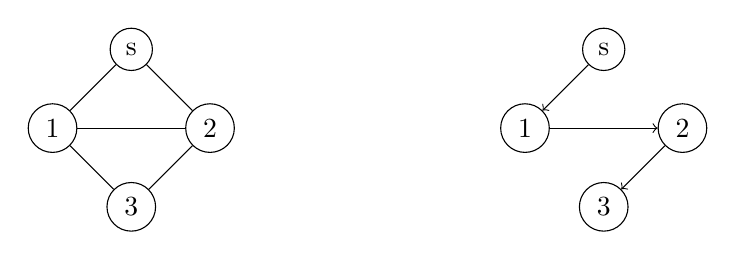
\begin{tikzpicture}[every node/.style={circle, draw, minimum width=5mm}]

\node(s) at(0,0) {s};
\foreach [count=\i] \x\y in {-1/-1,1/-1,0/-2}{
	\node(\i) at(\x,\y) {\i};
}

\foreach \u \v in {
s/1%
,s/2%
,1/2%
,1/3%
,2/3%
}{
	\draw (\u) -- (\v);
}

\begin{scope}[xshift=6cm]
\node(s) at(0,0) {s};
\foreach [count=\i] \x\y in {-1/-1,1/-1,0/-2}{
	\node(\i) at(\x,\y) {\i};
}

\foreach \u \v in {
s/1%
,1/2%
,2/3%
}{
	\draw[->] (\u) -- (\v);
}
\end{scope}

\end{tikzpicture}
\end{center}

